\documentclass{report}
\usepackage{tikz}
\usepackage{listings, listings-rust}
\usepackage{titlesec}
\setcounter{secnumdepth}{3}
\usetikzlibrary{fit}
\usepackage[toc,section=section]{glossaries}

\tikzset{
    vertex/.style={
        circle,
        fill    = blue,
        outer sep = 2pt,
        inner sep = 1pt,
    }
}

%opening
\title{%
    EDB: Debugger for Ethereum's Programming Languages \\
	\medskip
	\large Report \#4: System Design \\
    \large Advised by Dr. Jackowitz	\\
	\large University of Scranton}
\author{Andrew Plaza}

\begin{document}
\maketitle
\newpage

\begin{abstract}
    \begin{enumerate}
        \item Hello
    \end{enumerate}
\end{abstract}

\tableofcontents
\newpage

\section{Introduction}
    The EDB client application may be launched via the shell with the `edb' command, which launches the main program routine for the binary. Depending upon the options the user has passed EDB, the main program will first connect to the locally-run ethereum test node the user has setup, which EDB references throughout the rest of its execution. The solidity source code file that will be debugged must also be provided by the user. From these inputs EDB creates two of it's highest-level abstractions, the Compiler Model and the Emulator model, which make up the functionality of the debugger. The compiler model handles objects created by the compilation of the target source-language, such as the Abstract Syntax Tree, Source Mappings, and Bytecode. The Emulator model handles execution control and stores the Ethereum Virtual Machine(EVM) state at different steps in execution. State that is stored includes the current EVM Stack, Memory, and Non-Volatile Storage. Internally, the Emulator model uses the `sputnikvm' library. These parts make up the core of the debuggers functionality. Built on top of these items is also an optional JSON-RPC, which may be used in order to build featureful Graphical User Interfaces from 3rd-party applications.

    The design of EDB started first with a general development plan where models that were needed were identified. Based upon this plan, generic interfaces were created based upon the needs of the structure. Once this was complete, development was constrained to one part or sub-part of one model/interface, which worked towards fitting into the generic interface that was created during the first step. Unit tests were created alongside the original development of the part or sub-part, and testing took place to ensure the part worked individually before moving on to connect the part with the rest of the program. A kanban board on `Github Projects` was used in order to keep track of work that is under development, finished, or needs to be started.

\section{Levels}
\newpage
\subsection{High Level System Model}
\begin{center}
    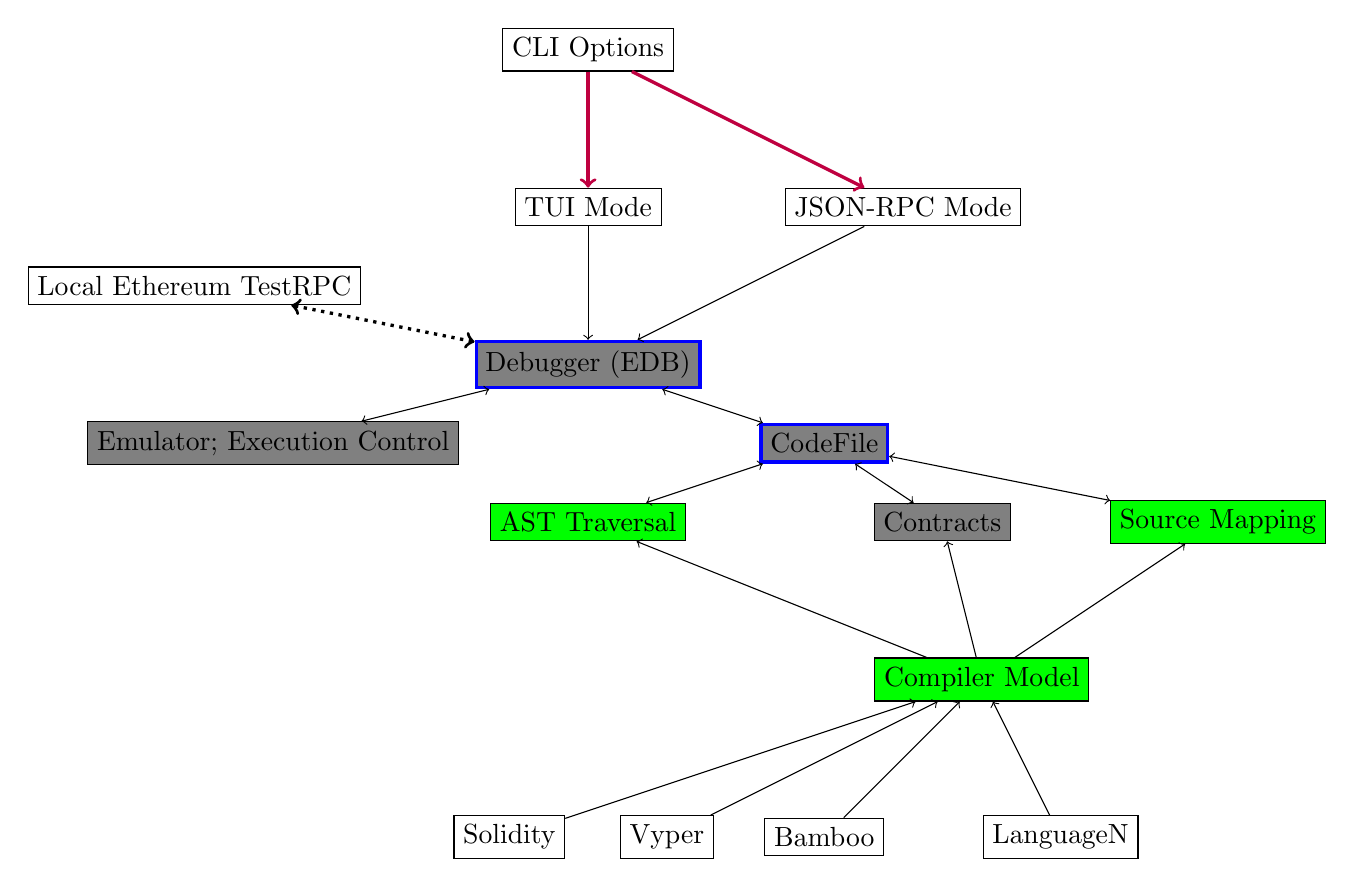
\begin{tikzpicture}



		\node[draw] (CLI) at (8,10) {CLI Options};

		\node[draw] (JSONRPC) at (12, 8) {JSON-RPC Mode};
		\node[draw] (TUIMode) at (8, 8) {TUI Mode};

		\node[draw] (ETH) at (3,7) {Local Ethereum TestRPC};

        \node[draw=blue,fill=gray,very thick] (EDB) at (8,6) {Debugger (EDB)};
        \node[draw,fill=gray] (EVM) at (4, 5) {Emulator; Execution Control};
        \node[draw=blue,fill=gray,very thick] (CodeFile) at (11,5) {CodeFile};
        %% Uh-Oh -- What creates the contracts? Not all three items there use the compiler. Only contracts/debug file
        \node[draw,fill=green] (AST) at (8, 4) {AST Traversal};
        \node[draw,fill=gray] (Contracts) at (12.5, 4) {Contracts};
        \node[draw,fill=green] (SrcMaps) at (16, 4) {Source Mapping};

        \node[draw,fill=green] (Compiler) at (13, 2) {Compiler Model};

        \node[draw] (Solidity) at (7, 0) {Solidity};
        \node[draw] (Vyper) at (9, 0) {Vyper};
        \node[draw] (Bamboo) at (11, 0) {Bamboo};
        \node[draw] (LanguageN) at (14,0) {LanguageN};

		\draw[->,draw=purple,very thick] (CLI) to (JSONRPC);
		\draw[->,draw=purple,very thick] (CLI) to (TUIMode);

		\draw[->,draw=black] (JSONRPC) to (EDB);
		\draw[->,draw=black] (TUIMode) to (EDB);


        \draw[<->,draw=black] (EDB) to (EVM);
        \draw[<->,draw=black] (EDB) to (CodeFile);
		\draw[<->,draw=black,dotted,very thick] (EDB) to (ETH);

        \draw[<->,draw=black] (CodeFile) to (AST);
        \draw[<->,draw=black] (CodeFile) to (SrcMaps);
        \draw[<->,draw=black] (CodeFile) to (Contracts);

        \draw[<-,draw=black] (AST) to (Compiler);
        \draw[<-,draw=black] (SrcMaps) to (Compiler);
        \draw[<-,draw=black] (Contracts) to (Compiler);

        \draw[->,draw=black] (Solidity) to (Compiler);
        \draw[->,draw=black] (Vyper) to (Compiler);
        \draw[->,draw=black] (Bamboo) to (Compiler);
        \draw[->,draw=black] (LanguageN) to (Compiler);
        %%% Color Legend
	\end{tikzpicture}
\end{center}
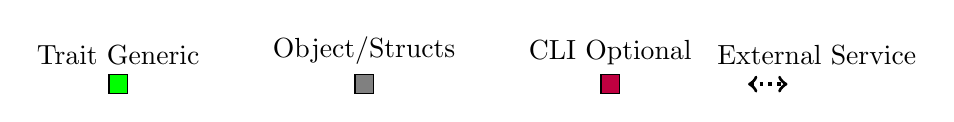
\begin{tikzpicture}
	\node [label=Trait Generic,draw,fill=green] (node1) {};
	\node [label={[name=l] Object/Structs},draw,fill=gray] (node2) at ([xshift=3cm]node1.east){};
	\node [label={[name=l] CLI Optional},draw,fill=purple] (node3) at ([xshift=3cm]node2.east){};
    \node [label={[name=l] External Service}] (node4) at ([xshift=2.5cm]node3.east){};
	\draw [<->,draw=black,dotted,very thick] (8,0) to (8.5,0);
\end{tikzpicture}
\vspace*{1cm}

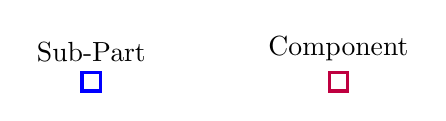
\begin{tikzpicture}
    \node [label=Sub-Part,draw=blue,very thick] (node1) {};
    \node [label={[name=l] Component},draw=purple, very thick] (node2) at ([xshift=3cm]node1.east){};
\end{tikzpicture}

\newpage

\subsection{CLI Options: TUI Mode, JSON-RPC Mode}
    \subsubsection{Abstract Specification}
    \subsubsection{Interface Design}
    \subsubsection{Component Design: TUI Mode}
    \subsubsection{Component Design: JSON-RPC Mode}

\subsection{Debugger Core}
    \subsubsection{Abstract Specification}
    \subsubsection{Interface Design}
    \subsubsection{Algorithm Design}
    \subsubsection{Data Structure Design}

\subsection{Emulator, Execution Control}
    \subsubsection{Abstract Specification}
    \subsubsection{Interface Design}
    \subsubsection{Algorithm Design}

\subsection{CodeFile}
    \subsubsection{Abstract Specification}
    \subsubsection{Interface Design}
    \subsubsection{}

\subsection{AST Traversal}
    \subsubsection{Abstract Specification}
    \subsubsection{Interface Design}

\subsection{Contracts}
    \subsubsection{Abstract Specification}
    \subsubsection{Interface Design}

\subsection{Source Mapping}
    \subsubsection{Abstract Specification}
    \subsubsection{Interface Design}

\subsection{Compiler}
    \subsubsection{Abstract Specification}
    \subsubsection{Interface Design}

\section{User Interface}

-- What To Do:
    - Provide a 'Abstract Spec' of every component (Debugger, Compilier, Source Map, AST, Contracts, CodeFile, etc)
        - provide data structs, and component design of every piece of that (graph it out. Graphs don't have to be as complicated as first. But enough to get the gist of the design of the compnonent)
        -

Test Rust Code
\begin{lstlisting}[language=Rust]
    pub trait Foo {
        fn killAllBunnies<F>(fun: F) -> AstItem
        where
            F: Fn(&mut AbstractFunction) -> bool;
        fn scrapeWebForSkynet();
    }
\end{lstlisting}
\section{Help System}

\section{}

\end{document}
